% !TeX root = RJwrapper.tex
\title{Modifying the Anhøj Rules to Improve Runs Analysis in Statistical
Process Control}
\author{by Jacob Anhøj, Tore Wentzel-Larsen}

\maketitle

\abstract{%
An abstract of less than 150 words.
}

% Any extra LaTeX you need in the preamble

\hypertarget{introduction}{%
\subsection{Introduction}\label{introduction}}

Within statistical process control (SPC) runs analysis is being used to
detect persistent shifts in process location over time.

We have previously shown that runs analysis using the Anhøj rules have
comparable or even better diagnostic properties than traditional control
chart rules that are commonly used to detect minor to moderate
\emph{persistens} shifts in process location \citep{anhoej2018}.

\hypertarget{methods}{%
\subsection{Methods}\label{methods}}

\hypertarget{results}{%
\subsection{Results}\label{results}}

\hypertarget{discussion}{%
\subsection{Discussion}\label{discussion}}

\hypertarget{conclusion}{%
\subsection{Conclusion}\label{conclusion}}

Here is a reference to Figure \ref{figure:box11}.

\begin{figure}[htbp]
  \centering
  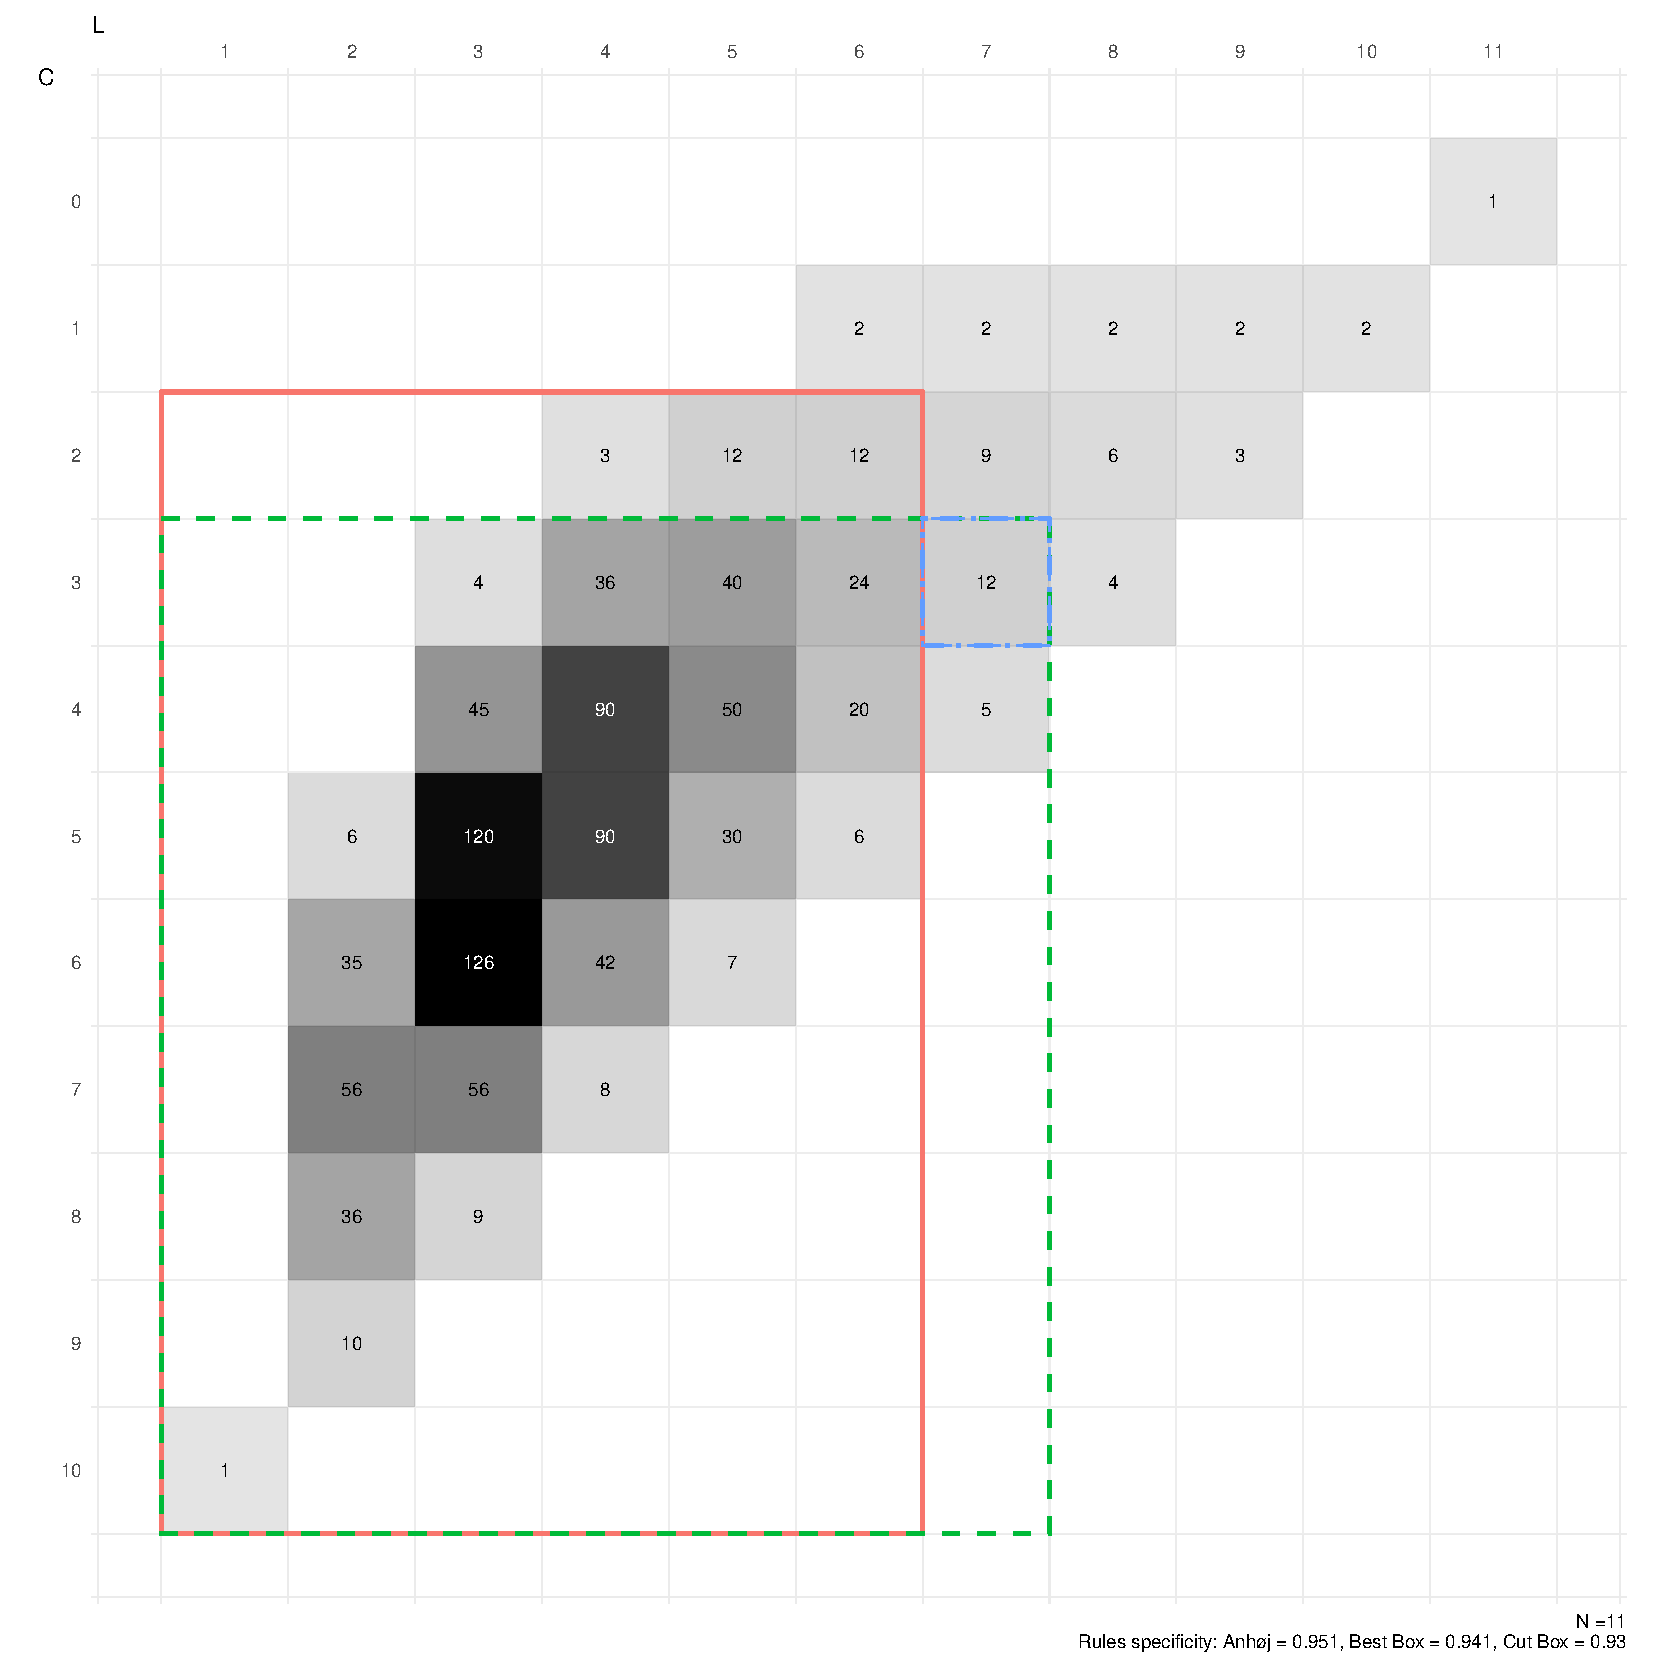
\includegraphics[width=\textwidth]{fig_box11.pdf}
  \caption{Borders of the anhøj, best box, and cut box rules.  
           The numbers in the cells are times representation of of the joint
           probabilities of longest run and number of crossings.}
  \label{figure:box11}
\end{figure}

Here is a reference to Figure \ref{figure:spec}.

\begin{figure}[htbp]
  \centering
  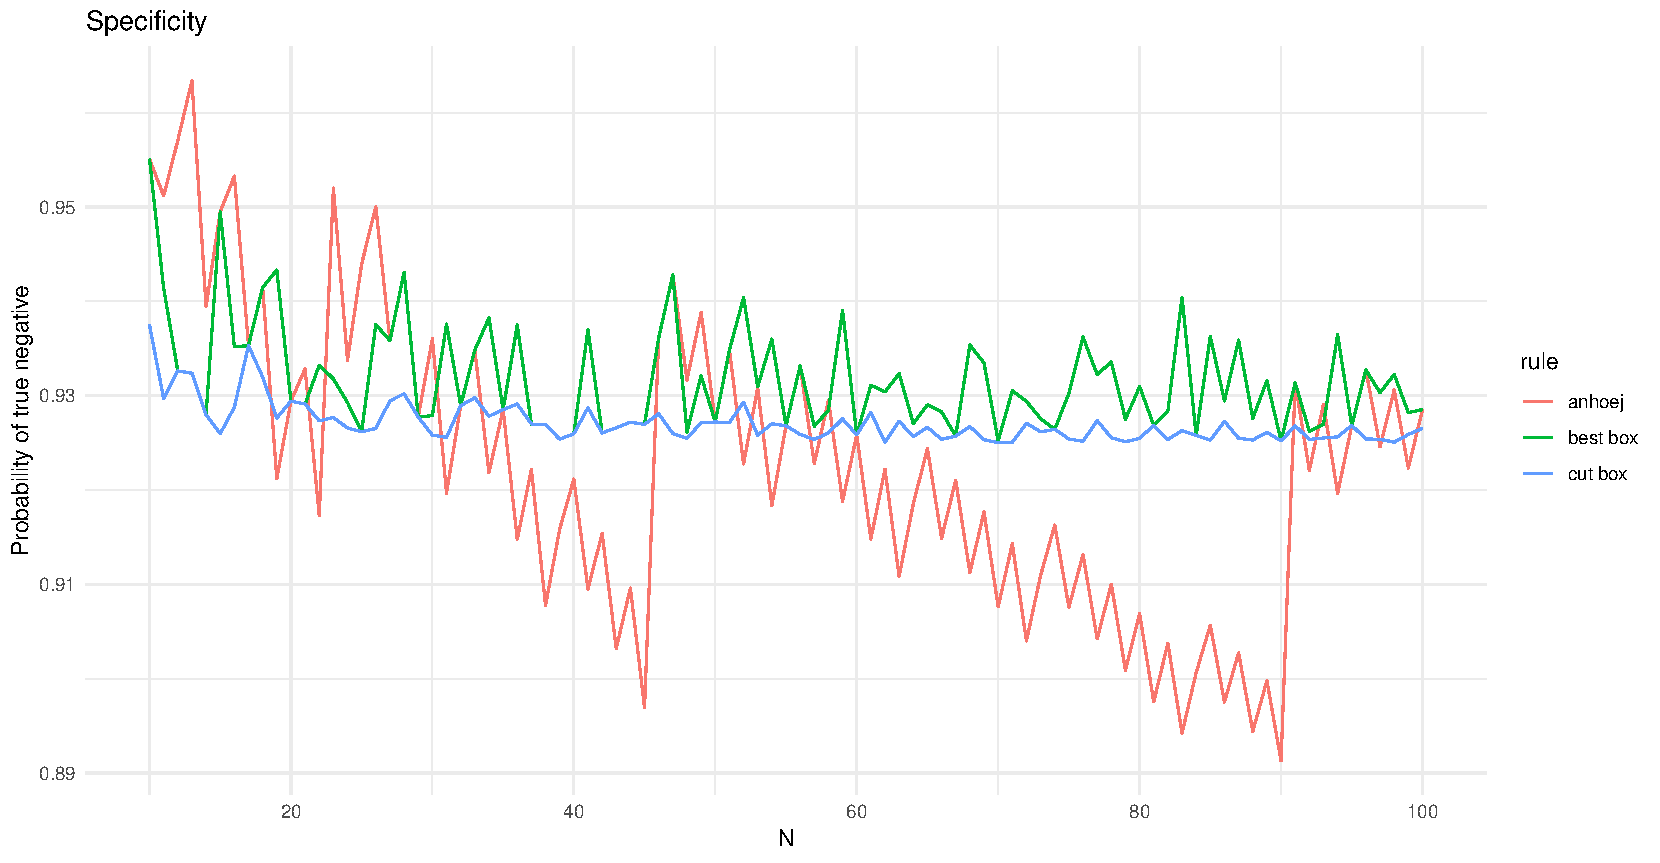
\includegraphics[width=\textwidth]{fig_spec.pdf}
  \caption{Specificity of the anhøj, best box, and cut box rules.}
  \label{figure:spec}
\end{figure}

Here is a reference to Figure \ref{figure:pwr}.

\begin{figure}[htbp]
  \centering
  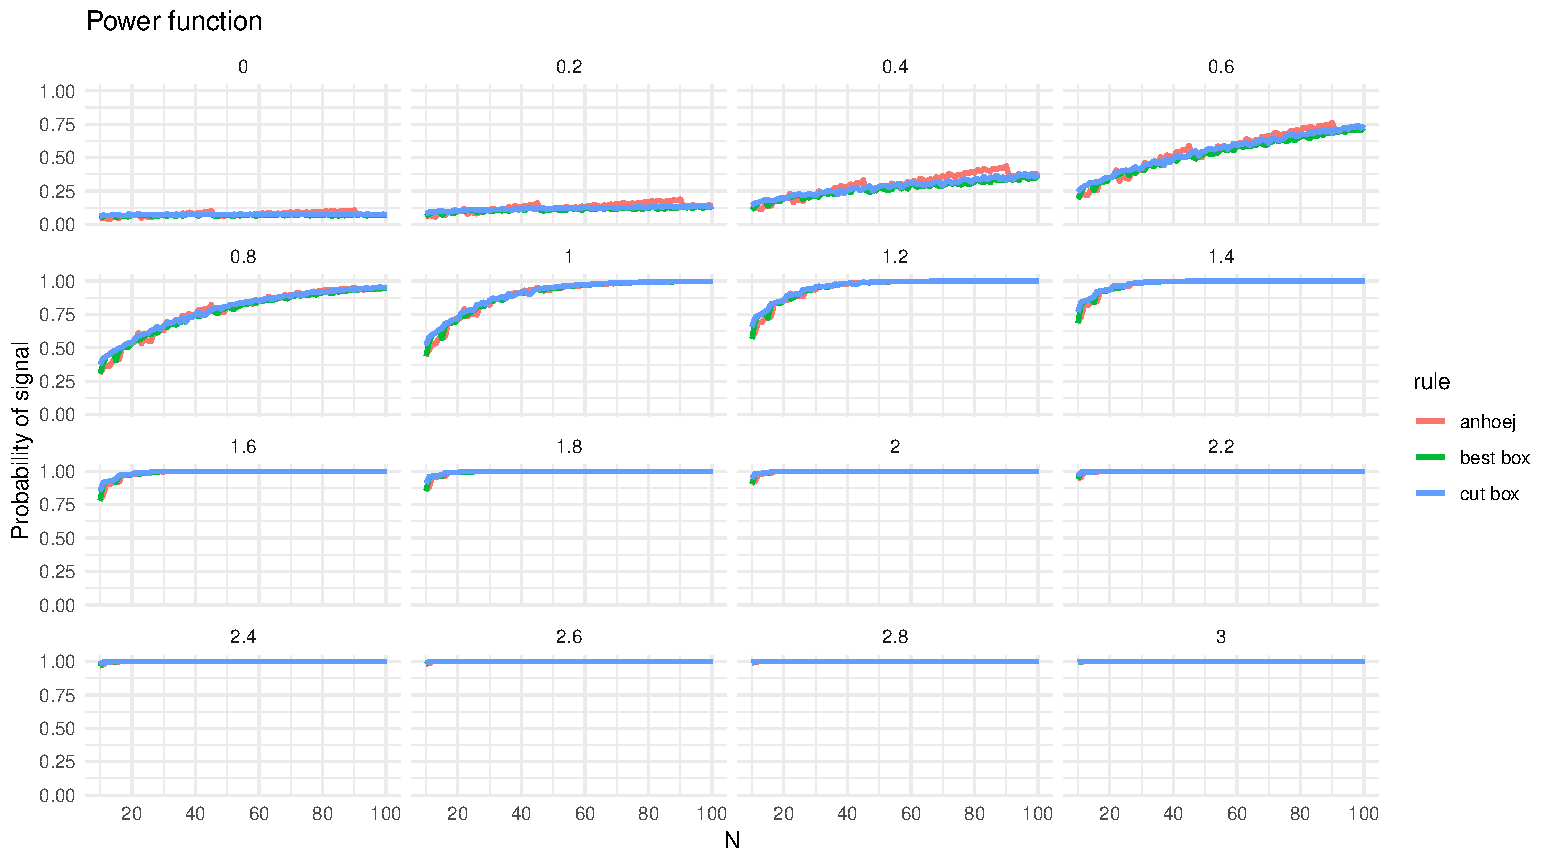
\includegraphics[width=\textwidth]{fig_pwr.pdf}
  \caption{Power function.}
  \label{figure:pwr}
\end{figure}

Here is a reference to Figure \ref{figure:lrpos}.

\begin{figure}[htbp]
  \centering
  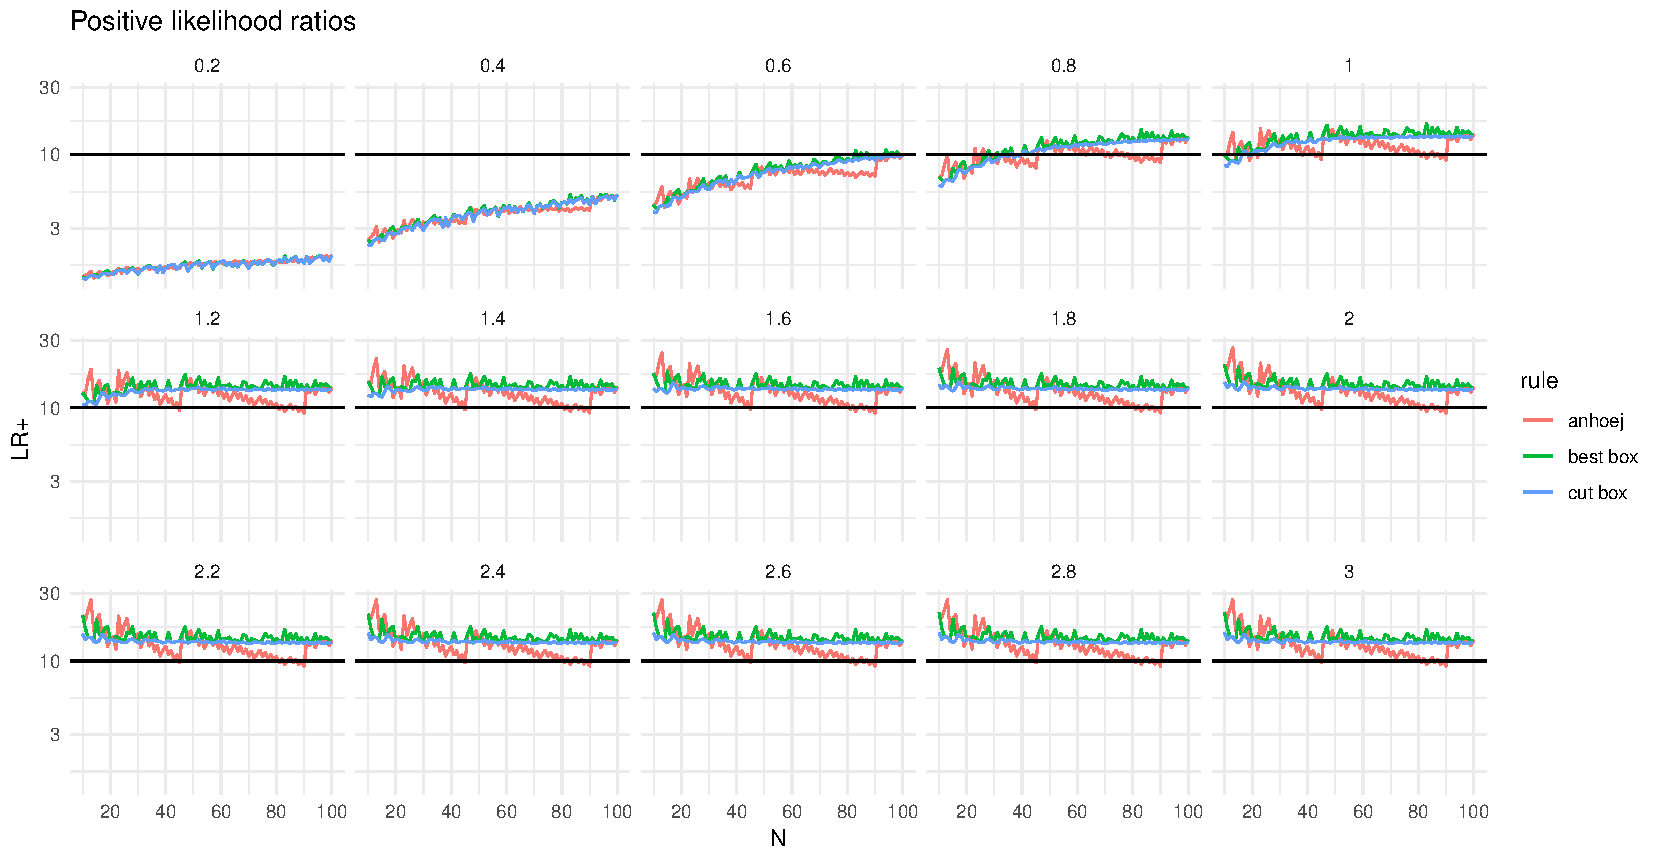
\includegraphics[width=\textwidth]{fig_lrpos.pdf}
  \caption{Positive likelihood ratio.}
  \label{figure:lrpos}
\end{figure}

Here is a reference to Figure \ref{figure:lrneg}.

\begin{figure}[htbp]
  \centering
  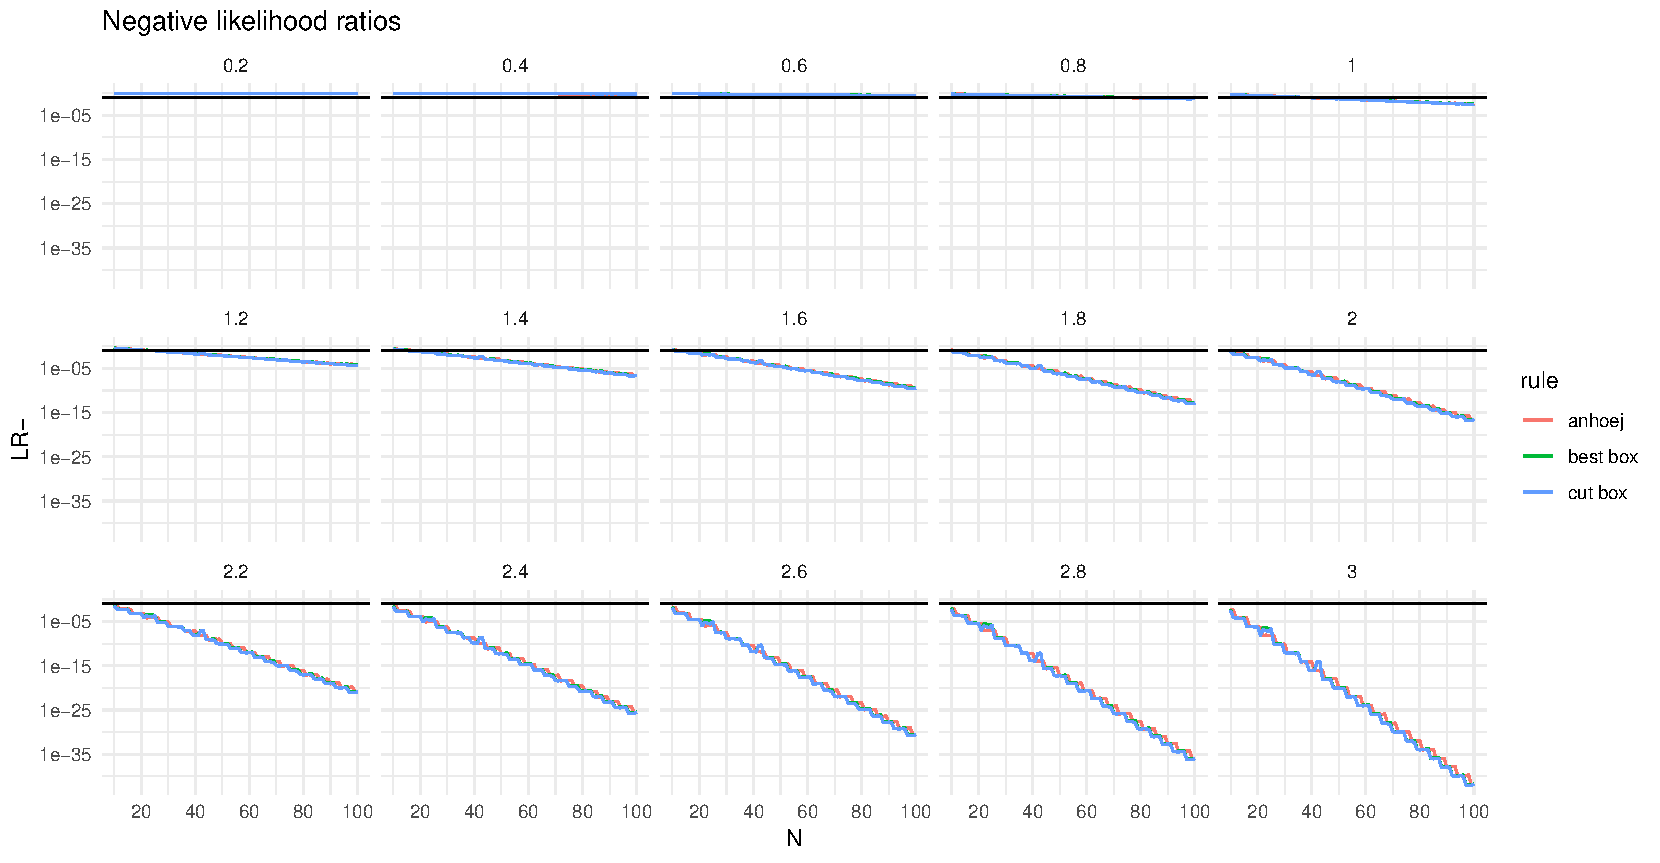
\includegraphics[width=\textwidth]{fig_lrneg.pdf}
  \caption{Negative likelihood ratio.}
  \label{figure:lrneg}
\end{figure}

\begin{Schunk}

\begin{longtable}{rrrrrrr}
\caption{\label{tab:unnamed-chunk-1}Signal limits for the anhøj and best box rules and borders for the cut
        box rules. N = number of trials. L = upper limit for longest run, 
        C = lower limit for number of crossings, Cbord and Lbord = cut box 
        borders to keep.}\\
\toprule
\multicolumn{1}{c}{ } & \multicolumn{2}{c}{Anhøj} & \multicolumn{2}{c}{Best box} & \multicolumn{2}{c}{Cut box} \\
\cmidrule(l{3pt}r{3pt}){2-3} \cmidrule(l{3pt}r{3pt}){4-5} \cmidrule(l{3pt}r{3pt}){6-7}
N & L & C & L & C & Cbord & Lbord\\
\midrule
\endfirsthead
\caption[]{Signal limits for the anhøj and best box rules and borders for the  \textit{(continued)}}\\
\toprule
\multicolumn{1}{c}{ } & \multicolumn{2}{c}{Anhøj} & \multicolumn{2}{c}{Best box} & \multicolumn{2}{c}{Cut box} \\
\cmidrule(l{3pt}r{3pt}){2-3} \cmidrule(l{3pt}r{3pt}){4-5} \cmidrule(l{3pt}r{3pt}){6-7}
N & L & C & L & C & Cbord & Lbord\\
\midrule
\endhead
\
\endfoot
\bottomrule
\endlastfoot
10 & 2 & 6 & 2 & 6 & 3 & 5\\
11 & 2 & 6 & 3 & 7 & 4 & 6\\
12 & 3 & 7 & 3 & 6 &  & \\
13 & 3 & 7 & 3 & 6 &  & \\
14 & 4 & 7 & 3 & 6 &  & \\
\addlinespace
15 & 4 & 7 & 4 & 7 & 6 & 6\\
16 & 4 & 7 & 5 & 8 & 6 & 7\\
17 & 5 & 7 & 5 & 7 &  & \\
18 & 5 & 7 & 5 & 7 & 6 & 6\\
19 & 6 & 7 & 5 & 7 & 6 & 5\\
\addlinespace
20 & 6 & 7 & 6 & 7 &  & \\
21 & 6 & 7 & 7 & 8 &  & \\
22 & 7 & 7 & 6 & 7 & 7 & 6\\
23 & 7 & 8 & 6 & 7 & 7 & 6\\
24 & 8 & 8 & 6 & 7 & 7 & 6\\
\addlinespace
25 & 8 & 8 & 6 & 7 &  & \\
26 & 8 & 8 & 9 & 9 & 10 & 7\\
27 & 9 & 8 & 9 & 8 & 10 & 7\\
28 & 9 & 8 & 9 & 8 & 11 & 7\\
29 & 10 & 8 & 10 & 8 &  & \\
\addlinespace
30 & 10 & 8 & 11 & 10 & 12 & 9\\
31 & 11 & 8 & 11 & 9 & 14 & 8\\
32 & 11 & 8 & 11 & 8 &  & \\
33 & 11 & 8 & 11 & 8 & 12 & 7\\
34 & 12 & 8 & 11 & 8 & 13 & 7\\
\addlinespace
35 & 12 & 8 & 12 & 8 &  & \\
36 & 13 & 8 & 13 & 9 & 15 & 8\\
37 & 13 & 8 & 14 & 10 &  & \\
38 & 14 & 8 & 13 & 8 &  & \\
39 & 14 & 8 & 15 & 11 &  & \\
\addlinespace
40 & 14 & 8 & 15 & 9 &  & \\
41 & 15 & 8 & 15 & 9 & 17 & 8\\
42 & 15 & 8 & 14 & 8 &  & \\
43 & 16 & 8 & 14 & 8 &  & \\
44 & 16 & 8 & 17 & 10 &  & \\
\addlinespace
45 & 17 & 8 & 17 & 9 &  & \\
46 & 17 & 9 & 17 & 9 & 19 & 8\\
47 & 17 & 9 & 17 & 9 & 20 & 7\\
48 & 18 & 9 & 19 & 12 & 20 & 11\\
49 & 18 & 9 & 19 & 10 & 21 & 9\\
\addlinespace
50 & 19 & 9 & 19 & 9 &  & \\
51 & 19 & 9 & 19 & 9 & 21 & 8\\
52 & 20 & 9 & 19 & 9 & 21 & 7\\
53 & 20 & 9 & 21 & 11 & 23 & 9\\
54 & 21 & 9 & 21 & 10 & 23 & 8\\
\addlinespace
55 & 21 & 9 & 21 & 9 &  & \\
56 & 21 & 9 & 21 & 9 & 23 & 8\\
57 & 22 & 9 & 23 & 12 & 25 & 11\\
58 & 22 & 9 & 23 & 10 & 24 & 9\\
59 & 23 & 9 & 23 & 10 & 26 & 8\\
\addlinespace
60 & 23 & 9 & 23 & 9 &  & \\
61 & 24 & 9 & 23 & 9 & 24 & 8\\
62 & 24 & 9 & 25 & 11 & 27 & 9\\
63 & 25 & 9 & 25 & 10 & 27 & 9\\
64 & 25 & 9 & 26 & 11 & 27 & 10\\
\addlinespace
65 & 25 & 9 & 26 & 10 & 27 & 9\\
66 & 26 & 9 & 27 & 12 & 29 & 10\\
67 & 26 & 9 & 27 & 10 &  & \\
68 & 27 & 9 & 27 & 10 & 29 & 8\\
69 & 27 & 9 & 28 & 11 & 29 & 8\\
\addlinespace
70 & 28 & 9 & 29 & 14 & 30 & 13\\
71 & 28 & 9 & 29 & 11 & 31 & 9\\
72 & 29 & 9 & 29 & 10 & 30 & 9\\
73 & 29 & 9 & 30 & 11 & 31 & 10\\
74 & 29 & 9 & 30 & 10 &  & \\
\addlinespace
75 & 30 & 9 & 31 & 12 & 32 & 9\\
76 & 30 & 9 & 31 & 11 & 34 & 8\\
77 & 31 & 9 & 31 & 10 & 33 & 9\\
78 & 31 & 9 & 32 & 11 & 33 & 8\\
79 & 32 & 9 & 33 & 13 & 37 & 11\\
\addlinespace
80 & 32 & 9 & 33 & 11 & 35 & 9\\
81 & 33 & 9 & 33 & 10 &  & \\
82 & 33 & 9 & 34 & 11 & 36 & 10\\
83 & 34 & 9 & 33 & 10 & 36 & 7\\
84 & 34 & 9 & 35 & 11 &  & \\
\addlinespace
85 & 34 & 9 & 35 & 11 & 38 & 8\\
86 & 35 & 9 & 35 & 10 & 36 & 9\\
87 & 35 & 9 & 35 & 10 & 38 & 8\\
88 & 36 & 9 & 37 & 12 & 38 & 10\\
89 & 36 & 9 & 37 & 11 & 39 & 9\\
\addlinespace
90 & 37 & 9 & 38 & 12 &  & \\
91 & 37 & 10 & 37 & 10 & 39 & 9\\
92 & 38 & 10 & 39 & 13 & 41 & 12\\
93 & 38 & 10 & 39 & 11 & 40 & 10\\
94 & 39 & 10 & 39 & 11 & 42 & 8\\
\addlinespace
95 & 39 & 10 & 39 & 10 &  & \\
96 & 39 & 10 & 39 & 10 & 41 & 8\\
97 & 40 & 10 & 41 & 12 & 42 & 9\\
98 & 40 & 10 & 41 & 11 & 44 & 9\\
99 & 41 & 10 & 42 & 12 & 43 & 10\\
\addlinespace
100 & 41 & 10 & 41 & 10 & 42 & 9\\*
\end{longtable}

\end{Schunk}

\bibliography{RJreferences}


\address{%
Jacob Anhøj\\
Rigshospitalet, University of Copenhagen\\
Denmark\\
}
\href{mailto:jacob@anhoej.net}{\nolinkurl{jacob@anhoej.net}}

\address{%
Tore Wentzel-Larsen\\
Centre for Child and Adolescent Mental Health, Eastern and Southern
Norway \& Centre for Violence and Traumatic Stress Studies, Oslo, Norway\\
Norway\\
}
\href{mailto:tore.wentzellarsen@gmail.com}{\nolinkurl{tore.wentzellarsen@gmail.com}}

